%%%%%%%%%%%%%%%%%%%%%%%%%%%%%%%%%%%%%%%%%%%%%%%%%%%%%%%%%%%%%%%%%%%%%%%%%%%%%%%%
\chapter{Distractor Node Generation}\label{sec:dn}

\begin{chapterBody}

\begin{figure}[ht]
    \centering
    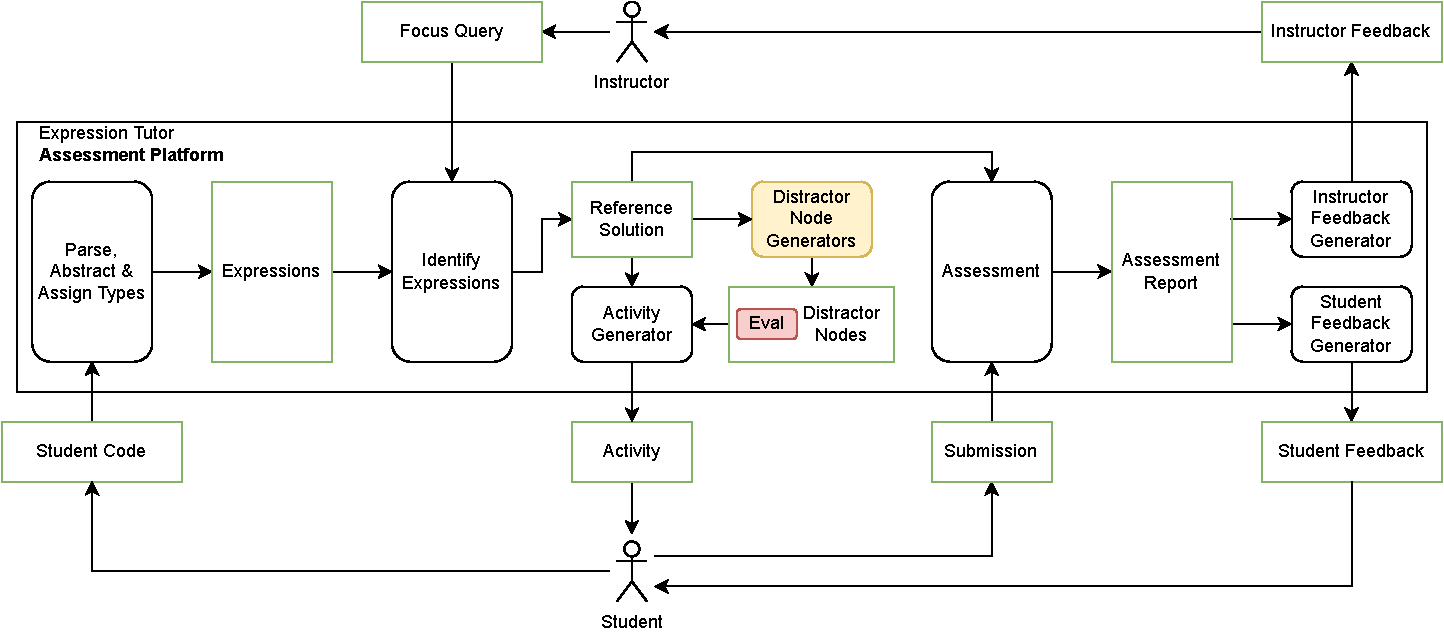
\includegraphics[width=\textwidth]{res/5/et_loop_distractors.pdf}
    \caption{Generating distractor nodes for the expression tree of a reference
solution.}
    \label{fig:dn-intro-loop}
\end{figure}

A properly designed notional machine should be usable regardless of the
platform or medium. Instructors may create an exercise and have students solve
it on paper by drawing the expression tree by hand. This puts the students in
an extremely free environment that poses no constraints on the tree that is
being drawn.

We look at past exams of a university–level course on object–oriented
programming. These exams included drawing expression trees as one of their
exercises. 
From the answers students provided, it can be seen that they may attempt to
construct all kinds of malformed trees.

For the implementation of the notional machine on the Expression Tutor platform
we want to offer a similar experience, while also leveraging all the benefits
that automation may bring. One such area in which automation can be useful is
the configuration of the initial state of the activities.
Generating a meaningful, non-empty initial state for Expression Tutor activities
is challenging. A curated initial state offers to students a good opportunity to
focus on the essential aspects of the process of building an expression tree,
as opposed to what they would be required to do on paper.
Since drawing nodes on the Expression Tutor website is time–consuming (as
outlined in Chapter~\ref{sec:etl}), the initial state contains all the nodes
required to build the correct tree. These nodes are disconnected from each
other and randomly ordered, offering an experience similar to that of Parsons
problems~\cite{parsons_parsons_2006}.
Moreover, type and value labels are removed so that students may fill those
values as part of the task to complete.
Suggestions for possible type labels that students should apply
to nodes are also generated alongside the activity.
These are surfaced when the student is typing the nodes of the expression
tree they are building. This helps the student stay focused on the primary goal
of the activity - to build the expression tree corresponding to the
given expression - while minimizing the opportunities for less meaningful
mistakes such as typos.

Displaying just the correct nodes in the initial state of the activity does not
allow to mirror the same experience one would have when performing this activity
on paper as there would be less opportunities for mistakes since all nodes are
already provided. We overcome this issue, with the automatic generation of
``distractor nodes''. To achieve this, we design and implement
distractor node generators (\textbf{Section~\ref{sec:dn-distractors-gen}}.
We formalize a distractor node generator as a function that takes an
expression tree diagram (of a reference solution) and produces a set
of \texttt{Node}s, as highlighted in
\textbf{Figure~\ref{fig:dn-intro-loop}}.

\[
\text{distractorNodesGenerator}:
\text{ExprTreeDiagram}
\rightarrow
\text{Set}\left[\text{Node}\right]
\]

\section{Distractor Nodes}\label{sec:dn-distractors}

We do not require students to create their own nodes in Expression Tutor
activities that we generate automatically. Instead, we provide a set of nodes
from which students have to select the nodes they need. We generate that set of
nodes by taking all the nodes that are in the automatically created reference
solution (the nodes that are needed to build the correct tree). We augment that
set with the so–called ``distractor nodes''.

On one hand, this allows to eliminate some of the drawbacks that the removal of
the \hfill\break time–consuming and typo–prone task of manually creating all of
the nodes would bring.
On the other hand, providing students large quantities of nodes as the starting
point for their solution, can easily become overwhelming and a lot of time would
be spent just finding for the desired node. This would be no better than having 
no nodes at all as a starting point.

\textbf{Figure~\ref{fig:dn-initial-state-diff}} showcases how distractor nodes
enrich the initial Activity state and provide opportunities for mistakes to 
students.

\begin{figure}[ht]
    \centering
    \begin{subfigure}[b]{0.45\textwidth}
    \includegraphics[width=\linewidth]
                    {res/5/intial_state_without_distractors.png}
    \caption{Correct nodes only.}
    \end{subfigure}
    \begin{subfigure}[b]{0.45\textwidth}
    \includegraphics[width=\linewidth]
                    {res/5/intial_state_with_distractors.png}
    \caption{Correct and distractor nodes.}
    \end{subfigure}
    \caption{Comparison of initial activity states with and without distractor
nodes for the Java expression
\lstinline[language=Java]{count == 0 ? b : fibIter(a + b, a, count - 1)}}
    \label{fig:dn-initial-state-diff}
\end{figure}

\section{Identifying What Distractors to Generate}\label{sec:dn-id}

% Mention that usage of student's data was approved (ask Igor)
To avoid generate too many distractors, we analyze two exercises from two
different exams.
The exams are from an university–level course on object–oriented programming
languages.
In these exercises, students were given code snippets. Within each code
snippet there exists an highlighted expression for which students
had to draw an expression tree on paper.
We compare the students' submissions against the reference solution
and catalogue all of the incorrect nodes that students drew.
Due to the variety of incorrect nodes found in the student's submissions
we grouped them in different categories. Each categories tries to capture one
kind of mistake that the student made while writing the incorrect node.
We catalogue 17 categories, as represented in
\textbf{Table~\ref{tab:dn-distractors-categories}}).

By analyzing these nodes, we build a way to automatically generate those
from the\hfill\break
top–occurring categories of mistakes. This allows us to capture the most
frequent mistakes that student happen to make due to some incorrect mental
model.
Table~\ref{tab:dn-distractors-categories} highlights the number of incorrect
nodes for each category (\textit{Occurrences} column) and details whether or not
a category was selected to be reproduced by our automatic distractor nodes
generator.

Certain categories, due to the nature of the mistakes they represent, cannot
be generated algorithmically. Examples of such categories would be the
\textit{Crazy} (nodes for which no clear mistake pattern could be identified), 
\textit{EvaledExpr} (nodes that contain the result of the evaluation of one
or more sub–expressions) and \textit{OtherCode} (nodes that refer to code that is
not part of the expression) categories.

\begin{table}[htb!]
\centering
\begin{tabular}{lllr}
\thead{Category} & \thead{Example} & \thead{Generated} & \thead{Occurrences} \\
Inline & \begin{lstlisting}[language=etl]
("a" "==" "null")
\end{lstlisting} & Yes & 68 \\
InlineHole & \begin{lstlisting}[language=etl]
(() "+" () "+" () "+" ())
\end{lstlisting} & Yes & 21 \\ 
Split & \begin{lstlisting}[language=etl]
(() ":" ())
\end{lstlisting} & Yes & 15 \\
EvaledExpr & \begin{lstlisting}[language=etl]
("\"D\"")
\end{lstlisting} & No & 13 \\
OtherCode & \begin{lstlisting}[language=etl]
("String" " " "s" "=")
\end{lstlisting} & No & 12 \\
Extract & \begin{lstlisting}[language=etl]
(() "." ())
\end{lstlisting} & Yes & 10 \\
Crazy & \begin{lstlisting}[language=etl]
("a[i]" "=" "NULL" "+" "0")
\end{lstlisting} & No & 10 \\
MissingHoles & \begin{lstlisting}[language=etl]
("+")
\end{lstlisting} & No & 9 \\
CharAsString & \begin{lstlisting}[language=etl]
("\"+\"")
\end{lstlisting} & No & 7 \\
CodeInString & \begin{lstlisting}[language=etl]
("\"" () " = \"")
\end{lstlisting} & No & 7 \\
NoParenMethodCall & \begin{lstlisting}[language=etl]
("id" ())
\end{lstlisting} & No & 5 \\
EmptyNode & \begin{lstlisting}[language=etl]
( )
\end{lstlisting} & No & 3 \\
Typo & \begin{lstlisting}[language=etl]
("aa")
\end{lstlisting} & No & 2 \\
MismatchParen & \begin{lstlisting}[language=etl]
("id" "(" ()))
\end{lstlisting} & No & 1 \\
No[]ArrayAcc & \begin{lstlisting}[language=etl]
("a" ())
\end{lstlisting} & No & 1 \\
SingleEqualsForEquality & \begin{lstlisting}[language=etl]
(() "=" ())
\end{lstlisting} & No & 1 \\
SingleHole & \begin{lstlisting}[language=etl]
( () )
\end{lstlisting} & No & 1 \\
\end{tabular}
\caption{Categories of incorrect nodes.}
\label{tab:dn-distractors-categories}
\end{table}

\section{Distractor Node Generators}\label{sec:dn-distractors-gen}

By looking at the different categories gathered from the manual analysis
(Table~\ref{tab:dn-distractors-categories}), the occurrences of each one and
how much correlated each category is to syntactical and semantic rules of
the specific programming language, we select a number of categories that
we try to re–create programmatically by using a distractor node generator.
An important constraint that we have to consider when designing and implementing
our generators is that we need to avoid the combinatorial explosion of the number
of generated distractors that would happen if one was to generate all possible
distractors.

We now describe six different distractor node generators we designed to 
generate nodes that would belong to the categories we identified in
Table~\ref{tab:dn-distractors-categories}.

\begin{itemize}
    \item \textbf{Extract NameUse} distractor node generator: for each node in
the input diagram, generate distractor nodes such that each NameUse instance in
the original node is replaced with a hole alongside nodes with a single content
element (being the NameUse instance).

\begin{minipage}{.45\linewidth}
Input diagram: \texttt{f(1)}
\begin{lstlisting}[language=etl]
(u"f" "(" ("1") ")")
\end{lstlisting}
Generated distractors:
\begin{lstlisting}[language=etl]
(() "(" () ")")
(u"f")
\end{lstlisting}
\end{minipage}
\hspace{.1\linewidth}
\begin{minipage}{.4\linewidth}
\includegraphics[height=6em]{res/5/dn_gen_extract.png}
\end{minipage}

    \item \textbf{Inline} distractor node generator: for each node in the
input diagram, generate up to two distractor nodes.
\begin{enumerate}
    \item 1–level of inlining: the content of the children are brought into the
parent (but not recursively).

\begin{minipage}{.45\linewidth}
Input diagram: \texttt{f(g(1))}
\begin{lstlisting}[language=etl]
(u"f" "(" (u"g" "(" ("1") ")") ")")
\end{lstlisting}
Generated distractor:
\begin{lstlisting}[language=etl]
(u"f" "(" u"g" "(" () ")" ")")
\end{lstlisting}
\end{minipage}
\hspace{.1\linewidth}
\begin{minipage}{.4\linewidth}
\includegraphics[height=8em]{res/5/dn_gen_inline_1.png}
\end{minipage}

    \item Flattened node (only if the tree originating from that node has depth
less than 4, to avoid an excessive number of distractor nodes to be generated):
the content of the children are brought into the parent recursively.

\begin{minipage}{.45\linewidth}
Input diagram: \texttt{f(g(1))}
\begin{lstlisting}[language=etl]
(u"f" "(" (u"g" "(" ("1") ")") ")")
\end{lstlisting}
Generated distractor:
\begin{lstlisting}[language=etl]
(u"f" "(" u"g" "(" "1" ")" ")")
\end{lstlisting}
\end{minipage}
\hspace{.1\linewidth}
\begin{minipage}{.4\linewidth}
\includegraphics[height=8em]{res/5/dn_gen_inline_1.png}
\end{minipage}

\end{enumerate}
    \item \textbf{Inline holes} distractor node generator: for each node in
the input diagram, generate nodes that have in–lined only the non–atomic 
children (they contain holes).

\begin{minipage}{.45\linewidth}
Input diagram: \texttt{1 + 2 + 3}
\begin{lstlisting}[language=etl]
((("1") "+" ("2")) "+" ("3"))
\end{lstlisting}
Generated distractor:
\begin{lstlisting}[language=etl]
(() "+" () "+" ())
\end{lstlisting}
\end{minipage}
\hspace{.1\linewidth}
\begin{minipage}{.4\linewidth}
\includegraphics[height=8em]{res/5/dn_gen_inline_hole.png}
\end{minipage}

    \item \textbf{Atomic inline} distractor node generator: for each node
in the input diagram, generate up to $ 2^H $ inline distractor nodes (where
$ H $ is the number of holes among the node contents). This is done for all
possible combinations. This is a variation of the \textbf{Inline}
distractor node generator that was designed due to the observed tendency of
inlining non–atomic nodes in the training data set. This helps cover more
potential \textit{inlined} distractors while avoiding overloading students
with too many distractor nodes.

\begin{minipage}{.45\linewidth}
Input diagram: \texttt{f(1, 2, 3 + 4)}
\begin{lstlisting}[language=etl]
(u"f" "(" ("1") "," ("2") ","
  (("3") "+" ("4")) ")")
\end{lstlisting}
Generated distractors:
\begin{lstlisting}[language=etl]
(u"f" "(" "1" "," () "," () ")")
(u"f" "(" () "," "2" "," () ")")
(u"f" "(" "1" "," "2" "," () ")")
("3" "+" ())
(() "+" "4")
("3" "+" "4")
\end{lstlisting}
\end{minipage}
\hspace{.1\linewidth}
\begin{minipage}{.4\linewidth}
\includegraphics[height=12em]{res/5/dn_gen_atomic_inline.png}
\end{minipage}

    \item \textbf{Quotes} distractor node generator: for each node in the
input diagram, generate distractor nodes in which textual content written
between quotes is replaced with a hole placed between quotes. Single–quotes
(\texttt{'}), double–quotes (\texttt{"}) and back–quotes (\texttt{`}) are
supported.

\begin{minipage}{.45\linewidth}
Input diagram 1: \texttt{"Hello world"}
\begin{lstlisting}[language=etl]
("\"Hello world\"")
\end{lstlisting}
Generated distractors:
\begin{lstlisting}[language=etl]
("\"" () "\"")
("Hello world")
\end{lstlisting}
\end{minipage}
\hspace{.1\linewidth}
\begin{minipage}{.4\linewidth}
\includegraphics[height=6em]{res/5/dn_gen_quotes_1.png}
\end{minipage}


Input diagram 2 (assuming the quotes are in separate node content elements):

\begin{minipage}{.45\linewidth}
\texttt{'Hello world'}
\begin{lstlisting}[language=etl]
("'" "Hello world" "'")
\end{lstlisting}
Generated distractors:
\begin{lstlisting}[language=etl]
("'" () "'")
("Hello world")
\end{lstlisting}
\end{minipage}
\hspace{.1\linewidth}
\begin{minipage}{.4\linewidth}
\includegraphics[height=6em]{res/5/dn_gen_quotes_2.png}
\end{minipage}

    \item \textbf{Split} distractor node generator: for each node in the input
diagram that matches the following pattern 
\lstinline[language=etl]{(() [/.+/ ()]+)}, generate $ H - 1 $ distractor nodes
where $ H $ is the number of holes in the node. Each one of these distractor
contains one hole, followed by one textual element from the original one,
followed again by another hole.

\begin{minipage}{.45\linewidth}
Input diagram: \texttt{b ? 1 : 2}
\begin{lstlisting}[language=etl]
((u"b") "?" ("1") ":" ("2"))
\end{lstlisting}
Generated distractors:
\begin{lstlisting}[language=etl]
(() "?" ())
(() ":" ())
\end{lstlisting}
\end{minipage}
\hspace{.1\linewidth}
\begin{minipage}{.4\linewidth}
\includegraphics[height=8em]{res/5/dn_gen_split.png}
\end{minipage}
\end{itemize}

\subsection{Avoiding Redundant Distractors While Allowing Meaningful Repetition}

It should be apparent how some of these generators may produce the same
distractor node from the same original node due to the structure of said node
and the \textit{nature} of the distractor that is being generated.
At the same time, we do not want to reveal to the student whether a node is a 
distractor node by showing an inadequate quantity of it. That would not allow
the construction of a tree with the same \textit{linearization}
(Section~\ref{sec:fb-assess-linearization}) and would force the
student to run into inconsistencies during tree building. These
inconsistencies, if noticed, would be a signal the student that something is
wrong, and the distractor node would be easily detected regardless of the
knowledge of the student.

As an example, consider the Java expression
\lstinline[language=Java]{id(a[i].toString())}
(and its respective expression tree seen in
\textbf{Figure~\ref{fig:dn-duplicate-1}}). For this expression, both the
\textit{Inline} and the \textit{InlineHole} distractor generators would create
the distractors 
\lstinline[language=etl]{("id" "(" () "." "toString" "(" ")" ")")} and
\lstinline[language=etl]{("id" "(" () "[" () "]" "." "toString" "(" ")" ")")}.
Since having two copies of the same distractors is not useful here, we need to
preserve only one copy of each. 

On the other hand, if let's consider the Java expression
\lstinline[language=Java]{a[i].toString() + b[i].toString()}
(and its respective expression tree seen in
\textbf{Figure~\ref{fig:dn-duplicate-2}}). For this expression,
the  \lstinline[language=etl]{(() "[" () "]" "." "toString" "(" ")" ")")} 
distractor node is generated twice. In this case, we do not want to get rid of
the two copies as one is needed to express the mistake for the \texttt{a} array
and the other for the \texttt{b} array.

\begin{figure}[htb!]
    \centering
    \includegraphics[width=.3\textwidth]{res/5/dn_example_duplicate_tree_1.png}
    \caption{Multiple distractor node generators will create the same distractor
from the same correct node.}
    \label{fig:dn-duplicate-1}
\end{figure}

\begin{figure}[htb!]
    \centering
    \includegraphics[width=.3\textwidth]{res/5/dn_example_duplicate_tree_2.png}
    \caption{Multiple distractor node generators will create the same distractor
from different correct node.}
    \label{fig:dn-duplicate-2}
\end{figure}

To this end, we define the identity of a distractor node by looking at the
following traits:

\begin{enumerate}
    \item Its contents (Children are considered as ``holes'' and their contents
are disregarded).
    \item If defined: its type and value.
    \item The identifier of the node it originated from (guaranteed to be unique
within an expression tree diagram).
\end{enumerate}

The inclusion of the last trait makes it so that two if two distractor
generators produce from the same original node two distractors with the same
type, value and contents, their identity is considered to be the same. On the
other hand a if distractor generator produces the same distractor from two
different original nodes, then these distractors are also considered to be
different.

To obtain a numeric value out of these traits to use it as the node
identifier, we compute the 32-Bit cyclic redundancy code (also known as
CRC32)~\cite{koopman_32-bit_2002} of their binary linearization. This value is
fast enough to compute and is sufficiently collision resistant for this
particular use–case. Moreover, the size of the produced value fits perfectly in
the memory that was already being allocated for node identifiers. This, in turn,
allows to plug back into existing infrastructure that relies on said identifier
for distinguishing nodes in an expression tree diagram.

\section{Evaluation}

For each of the exercises we used to source incorrect nodes written by
students, we have taken one third of the incorrect nodes as ``training set''.
Those were used as a reference to build the different algorithmic distractor
generators.
Then, for evaluation purposes, we take the remaining two–thirds of nodes and
use them as ``test set'' to assess the capabilities of our algorithmic distractor
node generation.

We generate the distractor nodes using all of the generators implemented as
described in Section~\ref{sec:dn-distractors-gen} and evaluate how many
nodes in the test set are being generated.

\subsection{Exam 1}

In exam 1, students were asked to draw the expression tree
for the following Java expression:

\begin{lstlisting}[language=java]
"a[i] = " + (a == null ? "X" : id(a[i].toString())) + '+' + 0;
\end{lstlisting}

Where:

\begin{itemize}
    \item \texttt{a} is a variable of type \texttt{Object[]}
    \item \texttt{i} is a variable of type \texttt{int}
    \item \texttt{id} is a Java method declared as
\texttt{String id(String x)}
\end{itemize}

We execute the distractor generators on the expression. The system 
generates 37 distractor nodes that cover 49\% of all of the
incorrect nodes found in the test set. The results are detailed
in \textbf{Table~\ref{tab:dn-distractors-eval-final}}.

In the first column, \textit{Category} refers to the categories that were
defined during the manual review of the exams (Section~\ref{sec:dn-id}).
\textit{Count} refers to the number of incorrect nodes found in the test set
that belong to said category.
The column \textit{{\% Over total}} represents the percentage of nodes that
belong to that particular category over all of the incorrect nodes in the test
set. The \textit{Generated} column, contains the number of incorrect nodes that
belong to the category that were also found among those automatically generated
by the system.
The column \textit{\% Gen. in Category} represents a percentage value of the
count of incorrect nodes that our distractor node generators were able to cover
among all those that belong to the category.
The \textit{\% Gen. over total} column represents the percentage of the number
of generated nodes for the specific category over the total number of incorrect
nodes in the test set.

The generators achieved good results in the \texttt{MissingHoles}, 
\texttt{Inline} and \texttt{Split} categories. In particular, in the
\texttt{Inline} category, which is the largest one overall.
The \texttt{Extract} and \texttt{InlineHole} categories performed less well due
to the limitations imposed by the requirements of generating a limited amount of
distractors.
The categories for which there are 0 generated nodes are either those with lower
\textit{Count} value or those that cannot be generated by the distractor node
generators (such as the \texttt{Crazy} and \texttt{OtherCode} categories).

\begin{table}[htb!]
\centering
\begin{tabular}{lrrrrr}
\thead{Category} & \thead{Count} & \thead{\% Over total} &
\thead{Generated} & \thead{\% Gen. in Category} & \thead{\% Gen. over total} \\
SingleHole              &  1 &  1\% &  1 & 100\% &  1\% \\
MissingHoles            &  9 &  4\% &  8 &  89\% &  4\% \\
Inline                  & 68 & 34\% & 59 &  87\% & 30\% \\
Split                   & 15 &  7\% & 13 &  87\% &  6\% \\
MissingQuotes           &  9 &  4\% &  7 &  78\% &  4\% \\
CodeInString            &  7 &  3\% &  2 &  29\% &  1\% \\
Extract                 & 10 &  5\% &  2 &  20\% &  1\% \\
InlineHole              & 21 & 10\% &  4 &  19\% &  2\% \\
Crazy                   & 10 & 10\% &  0 &   0\% &  0\% \\
EvaledExp               & 13 &  6\% &  0 &   0\% &  0\% \\
OtherCode               & 12 &  6\% &  0 &   0\% &  0\% \\
ChasAsString            &  7 &  3\% &  0 &   0\% &  0\% \\
NoParenMethodCall       &  5 &  2\% &  0 &   0\% &  0\% \\
Typo                    &  2 &  1\% &  0 &   0\% &  0\% \\
EmptyNode               &  3 &  1\% &  0 &   0\% &  0\% \\
ParsedString            &  2 &  1\% &  0 &   0\% &  0\% \\
SingleEqualsForEquality &  1 &  1\% &  0 &   0\% &  0\% \\
No[]ArrayAcc            &  1 &  1\% &  0 &   0\% &  0\% \\
MismatchParen           &  0 &  0\% &  0 &     - &  0\% \\
\hline
\textbf{Total} & 196 & 100\% & 96 & & 49\% \\
\end{tabular}
\caption{Results for Exam 1.}
\label{tab:dn-distractors-eval-final}
\end{table}

\subsection{Exam 2}

In exam 2, students were asked to draw the expression tree for the following Java
expression:

\begin{lstlisting}[language=java]
publish(make("this"), make("that"))
\end{lstlisting}

Where:

\begin{itemize}
    \item \texttt{publish} is a Java method declared as
\texttt{String publish(String a, String b)}
    \item \texttt{make} is a Java method declared as
\texttt{String make(String target)}
\end{itemize}

For exam 2, the system generated 18 distractor nodes that cover 25\% of all of the
incorrect nodes found in the test set, as detailed by
\textbf{Table~\ref{tab:dn-distractors-eval-midterm}}.

The columns of this table are identical to those of
Table~\ref{tab:dn-distractors-eval-midterm}.
The generators achieved good results in the \texttt{Inline}, \texttt{CodeInString}
and \texttt{Extract} categories.
The results are different from those of the other exam. This can be attributed
to the different constructs contained in the expression that students had to
draw an expression tree for.
The distractor node generators perform significantly worse in Exam 2
due to the fact that over half of the incorrect nodes in the test set
belong to categories that cannot be reliably generated programmatically just by
looking at the expression tree of the expression in a language–agnostic way
(namely the \texttt{OtherCode}, \texttt{NoParenMethodCall}, \texttt{Typo} and
\texttt{Crazy}). 
For instance, in the second Exam, the presence of non–qualified method invocations
led many students to include the body of these invoked methods inside their
expression tree. These nodes are found in the \texttt{OtherCode} category and
this fact explains the high number of nodes in that category.

A considerable number of categories are also unused, some of which would have
been covered by the system if there was some construct in the expression
that offered an opportunity for said mistake.

These results highlight the complexity of the problem of generating distractor
nodes from a reference solution. The constructs involved in the \textit{original
expression} can influence which categories of mistakes can happen. This is
directly reflected in the performance of our algorithmic distractor node
generator as it was designed to cover a limited number of categories to
avoid the combinatorial explosion in number of generated distractor nodes.

\begin{table}[htb!]
\centering
\begin{tabular}{lrrrrr}
\thead{Category} & \thead{Count} & \thead{\% Over total} &
\thead{Generated} & \thead{\% Gen. in Category} & \thead{\% Gen. over total} \\
Inline                  &  7 &  9\% & 7 & 100\% & 9\% \\
CodeInString            &  6 &  8\% & 6 & 100\% & 8\% \\
Extract                 & 16 & 20\% & 7 &  43\% & 9\% \\
OtherCode               & 31 & 39\% & 0 &   0\% & 0\% \\
NoParenMethodCall       &  8 & 10\% & 0 &   0\% & 0\% \\
Typo                    &  5 &  6\% & 0 &   0\% & 0\% \\
MissingQuotes           &  4 &  5\% & 0 &   0\% & 0\% \\
Crazy                   &  1 &  1\% & 0 &   0\% & 0\% \\
MismatchParen           &  1 &  1\% & 0 &   0\% & 0\% \\
InlineHole              &  0 &  0\% & 0 &     - & 0\% \\
EvaledExp               &  0 &  0\% & 0 &     - & 0\% \\
EmptyNode               &  0 &  0\% & 0 &     - & 0\% \\
ChasAsString            &  0 &  0\% & 0 &     - & 0\% \\
ParsedString            &  0 &  0\% & 0 &     - & 0\% \\
Split                   &  0 &  0\% & 0 &     - & 0\% \\
SingleEqualsForEquality &  0 &  0\% & 0 &     - & 0\% \\
No[]ArrayAcc            &  0 &  0\% & 0 &     - & 0\% \\
MissingHoles            &  0 &  0\% & 0 &     - & 0\% \\
SingleHole              &  0 &  0\% & 0 &     - & 0\% \\
\hline
\textbf{Total} & 79 & 100\% & 20 & & 26\% \\
\end{tabular}
\caption{Results for Exam 2.}
\label{tab:dn-distractors-eval-midterm}
\end{table}
\end{chapterBody}
